\documentclass[11pt]{article}

\usepackage[a4paper,margin=1in]{geometry}
\usepackage{amsmath,amssymb,amsthm,mathtools}
\usepackage{graphicx}
\usepackage{float}
\usepackage{microtype}
\usepackage{xcolor}
\usepackage{enumitem}
\usepackage[colorlinks=true,linkcolor=blue!55!black,citecolor=blue!55!black,urlcolor=blue!60!black]{hyperref}

\newtheorem{theorem}{Theorem}
\newtheorem{corollary}{Corollary}
\newcommand{\one}{\mathbf 1}
\newcommand{\R}{\mathcal R}
\newcommand{\dom}{\operatorname{dom}}
\newcommand{\spb}{\operatorname{s}}

\title{A Rank-One Counterexample to the Domain-Free\\Ces\`aro/Maximum/Anti-Maximum Equivalence}
\author{Automated mathematics run \texttt{fa\_banach\_001}\\Lane 6 --- candidate for human review}
\date{9 August 2026}

\begin{document}
\maketitle

\begin{center}
\fbox{\parbox{0.91\textwidth}{\textbf{Status.}
Candidate counterexample, likely valid.  The result completely disproves the
literal extension of source Theorem~5.2 obtained by deleting
$\dom(A)\subseteq E_u$.  It does not completely resolve the source's broader
program of characterizing all relations between resolvent and Ces\`aro
positivity.}}
\end{center}

\section{Source question and exact scope}

Arora and Gl\"uck's Theorem~5.2 gives, under $\dom(A)\subseteq E_u$, a
four-way equivalence among eventual strong positivity of Ces\`aro means,
strong positivity of the spectral projection, an individual strong maximum
principle, and an individual strong anti-maximum principle
\cite[Theorem~5.2]{AroraGlueck2023}.  On PDF page~18 they ask for a better
understanding of the relation between resolvent and Ces\`aro positivity when
the domain inclusion is not imposed.

\begin{figure}[H]
  \centering
  
\includegraphics[width=0.82\textwidth]{figures/open_problem_crop.png}
  \caption{Source page~18: the end of Theorem~5.2 and the future-work
  direction concerning removal of $\dom(A)\subseteq E_u$.}
\end{figure}

The precise question settled here is the sharp literal one: can the domain
hypothesis simply be deleted while retaining the four-way equivalence?  The
answer is no, even for a bounded generator of a positive semigroup.  In fact,
conditions (i)--(iii) of the source theorem hold and condition (iv) fails.

\section{Definitions}

Let $E$ be a complex Banach lattice and $0<u\in E$.  Its principal ideal is
\[
 E_u=\{g\in E: |g|\leq c u\text{ for some }c\geq0\}.
\]
For real vectors $g,h$, write $g\succeq h$ if $g\geq c h$ for some $c>0$.
A positive $u$ is quasi-interior when $E_u$ is dense in $E$.

For a real $C_0$-semigroup $(e^{tA})_{t\geq0}$, its Ces\`aro mean at $r>0$ is
\[
 C(r)=\frac1r\int_0^r e^{tA}\,dt.
\]
The means are individually eventually strongly positive with respect to $u$
if, for every $0<f\in E$, one has $C(r)f\succeq u$ for all sufficiently
large $r$.  At a real pole $\lambda_0$, the individual strong maximum and
anti-maximum principles require the corresponding strong order inequalities
for $\R(\lambda,A)f$ on a right, respectively left, $f$-dependent
neighbourhood of $\lambda_0$.

\section{Idea of the proof}

Use the averaging projection $P f=(\int f)\one$ and put $A=P-I$.  The
semigroup and every Ces\`aro mean are convex combinations of $I$ and $P$,
so the positive rank-one part supplies an explicit lower bound by $\one$.
The right resolvent has the same favourable sign pattern.  On the left of the
pole, however, the identity coefficient is positive while the rank-one
coefficient is negative.  A positive unbounded $L^2$ function therefore
escapes every upper bound by a negative multiple of $\one$.  This is exactly
the regularity obstruction hidden by $\dom(A)\subseteq E_u$.

\section{Counterexample}

\begin{theorem}\label{thm:counterexample}
Let $E=L^2(0,1;\mathbb C)$ with its usual Banach-lattice order, let
$u=\one$, and define
\[
 \varphi(f)=\int_0^1 f(s)\,ds,\qquad Pf=\varphi(f)\one,\qquad A=P-I.
\]
Then:
\begin{enumerate}[label=\textup{(\roman*)}]
  \item $A$ generates a bounded positive uniformly continuous semigroup,
  $\spb(A)=0$ is a simple pole of the resolvent, and its spectral projection
  is $P$;
  \item the Ces\`aro means are strongly positive with respect to $u$ for
  every $r>0$;
  \item $Pf\succeq u$ for every $0<f\in E$;
  \item the individual strong maximum principle holds at $0$, in fact on
  the entire interval $(0,\infty)$;
  \item the individual strong anti-maximum principle at $0$ fails.
\end{enumerate}
Moreover, $\dom(A)=E\not\subseteq E_u$.  Hence assertions (i)--(iii) of
Arora--Gl\"uck Theorem~5.2 hold while assertion (iv) fails after the domain
hypothesis is removed.
\end{theorem}

\begin{proof}
Since $\varphi(\one)=1$, the positive rank-one operator $P$ is a projection.
Also $u=\one$ is quasi-interior and
\[
 E_u=L^\infty(0,1)\subsetneq L^2(0,1)=\dom(A).
\]
Because $P$ and $I-P$ are complementary projections,
\[
 A=0\cdot P-1\cdot(I-P),
 \qquad \sigma(A)=\{0,-1\}.
\]
Thus $0=\spb(A)$ is a simple pole and $P$ is its spectral projection.

Functional calculus for the two complementary projections gives
\[
 e^{tA}=P+e^{-t}(I-P)
       =e^{-t}I+(1-e^{-t})P.                         \tag{1}
\]
This is positive for every $t\geq0$ and bounded uniformly in $t$.  Integrating
(1), we obtain
\[
 C(r)=a_r I+(1-a_r)P,
 \qquad a_r=\frac{1-e^{-r}}r\in(0,1)                \tag{2}
\]
for every $r>0$.  If $0<f\in E$, strict positivity of integration on
$L^2_+$ gives $\varphi(f)>0$.  Hence
\[
 C(r)f\geq(1-a_r)\varphi(f)\one\succeq\one,
 \qquad Pf=\varphi(f)\one\succeq\one.              \tag{3}
\]
This proves the Ces\`aro and spectral assertions.  Notice that the lower
bound in (3) can even be made uniform for all $r\geq r_0>0$.

For $\lambda\notin\{-1,0\}$, decomposition along $P$ and $I-P$ yields
\begin{align}
 \R(\lambda,A)
 &=\frac1\lambda P+\frac1{\lambda+1}(I-P)\notag\\
 &=\frac1{\lambda+1}I
   +\frac1{\lambda(\lambda+1)}P.                    \tag{4}
\end{align}
If $\lambda>0$ and $0<f\in E$, both coefficients in the last line are
positive, and therefore
\[
 \R(\lambda,A)f\geq
 \frac{\varphi(f)}{\lambda(\lambda+1)}\one.
\]
This proves the individual strong maximum principle (and its usual scaled
form uniformly on every interval $(0,\varepsilon)$).

Now take the fixed positive vector
\[
 f(x)=x^{-1/4}\in L^2(0,1),\qquad \varphi(f)=\frac43.
\]
For every $\mu\in(-1,0)$, (4) gives
\[
 \R(\mu,A)f(x)
 =\frac1{1+\mu}\left(x^{-1/4}-\frac{4}{3|\mu|}\right). \tag{5}
\]
The right-hand side tends to $+\infty$ as $x\downarrow0$.  In particular it
is positive on a set of positive measure, so it is not $\leq0$ and a fortiori
cannot satisfy $\R(\mu,A)f\preceq-\one$.  The same fixed $f$ fails for every
$\mu\in(-1,0)$, which rules out every left neighbourhood of the pole.  This
proves the anti-maximum failure and completes the proof.
\end{proof}

\begin{corollary}
The domain hypothesis in source Theorem~5.2 cannot be omitted, even if one
strengthens the ambient assumptions by requiring $A$ to be bounded and the
semigroup to be positive for every time.
\end{corollary}

\section{Audit of the previously printed rank-one example}

The same operator on $L^2(0,1)$ appears on PDF page~3 of
Arora--Gl\"uck, arXiv:2203.05680v2 \cite{AroraGlueck2022}.  The displayed
resolvent formula there agrees with (4), but the following operator
anti-maximum inequality asserted in that passage does not.

\begin{figure}[H]
  \centering
  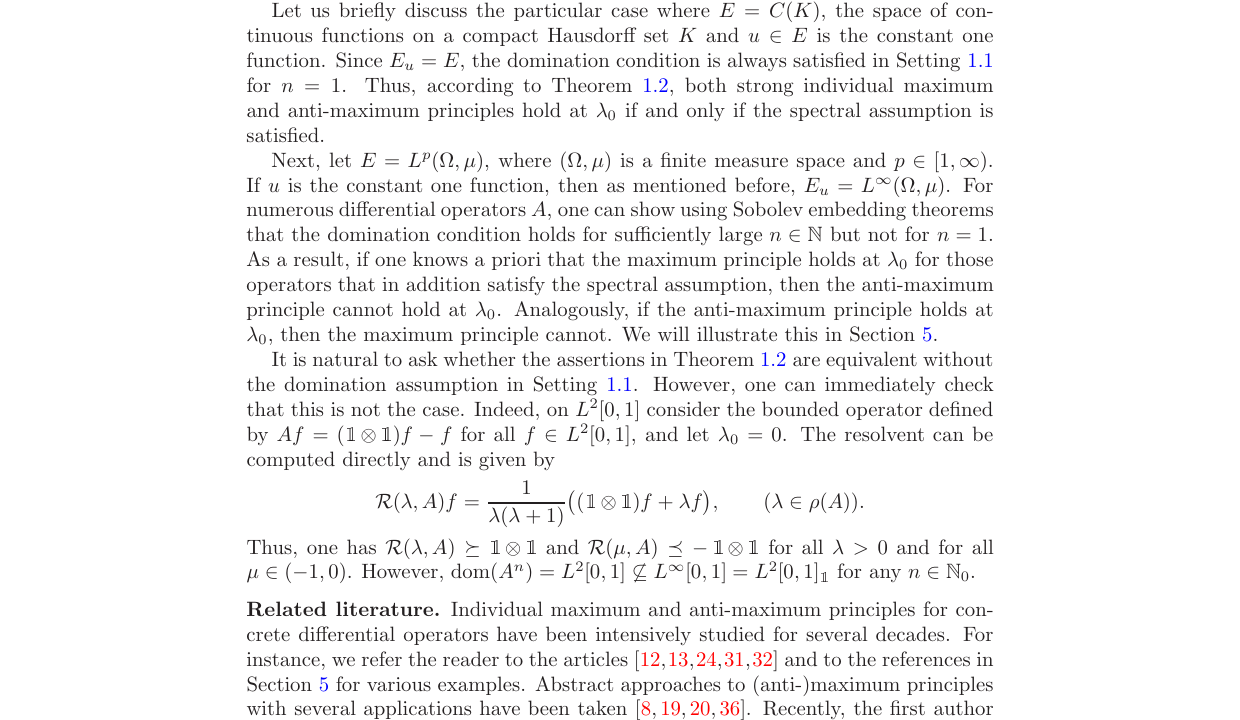
\includegraphics[width=\textwidth]{figures/literature_audit_crop.png}
  \caption{Supporting-paper page~3: the rank-one passage under audit.}
\end{figure}

Indeed, at $\mu=-\tfrac12$, formula (4) becomes
\[
 \R(-\tfrac12,A)=2I-4P.
\]
For the vector $f(x)=x^{-1/4}$ used above,
\[
 \R(-\tfrac12,A)f=2x^{-1/4}-\frac{16}{3},
\]
which is positive whenever $0<x<(3/8)^4$.  Thus this vector disproves even
ordinary anti-maximum negativity.  The issue is confined to this auxiliary
example: Theorem~1.2 of that paper assumes a weaker domination condition
$\dom(A^n)\subseteq E_u$ for some $n$, whereas the bounded operator here has
$\dom(A^n)=L^2(0,1)\not\subseteq L^\infty(0,1)$ for every $n\geq0$.

\section{Verification and limitations}

The proof was checked independently in four decomposed steps: projection and
spectrum, semigroup/Ces\`aro formula, resolvent formula, and the single-vector
order obstruction.  At $\mu=-1/2$ the calculation reduces to the especially
transparent identity $2I-4P$.  All conclusions are exact and require no
numerical experiment.

The bounded novelty search covered the local run indexes and full-source
corpus, the two cited arXiv records, exact title/id searches, close keyword
searches, and erratum/correction searches.  No later correction or exact
statement of this packet's conclusion was found as of 9 August 2026.  The
construction itself is printed in \cite{AroraGlueck2022}; the candidate-new
content is the corrected order analysis and its use against the domain-free
extension of \cite[Theorem~5.2]{AroraGlueck2023}.

This is not a full characterization of the broad future-work direction.  In
this example both the Ces\`aro means and the right-hand resolvent are strongly
positive, so it does not separate those two properties.  It proves the sharp
negative statement that those properties and strong spectral positivity do
not recover the anti-maximum conclusion without domain regularity.

\paragraph{Human review focus.}
Check (5), the order quantifiers on the whole interval $(-1,0)$, and the scope
of the literature-audit statement.  The candidate mathematical result is
recommended for promotion after those checks.

\begin{thebibliography}{9}
\bibitem{AroraGlueck2023}
S.~Arora and J.~Gl\"uck,
\emph{Criteria for eventual domination of operator semigroups and resolvents},
Operator Theory: Advances and Applications 292 (2023), 1--26;
\href{https://arxiv.org/abs/2204.00146}{arXiv:2204.00146v3}.

\bibitem{AroraGlueck2022}
S.~Arora and J.~Gl\"uck,
\emph{A characterization of the individual maximum and anti-maximum principle},
Math. Z. 305 (2023), article 49;
\href{https://arxiv.org/abs/2203.05680}{arXiv:2203.05680v2}.
\end{thebibliography}

\end{document}
